\documentclass{beamer}
 
\usepackage[utf8]{inputenc}
\usepackage[brazil]{babel} % pacote portugues brasileiro
\usepackage{textpos}
\usepackage{hyperref}
\definecolor{blue(pigment)}{rgb}{0.2, 0.2, 0.6}
\hypersetup{
    colorlinks=true,
    linkcolor=blue(pigment),
    filecolor=magenta,      
    urlcolor=cyan,
}
\usetheme{Montpellier}
\usecolortheme{rose}
% \graphicspath{{../../../2021-1/DesWebBasico/aulas/fig/}}
% Layout da pagina
\hypersetup{pdfpagelayout=SinglePage}
 
%Information to be included in the title page:
\title[HTML + CSS]{Formulários HTML}
 \subtitle{Disciplina: Desenvolvimento de Sistemas com PHP}
\author{Juliana C. Silva}
\institute{Universidade Positivo}

\definecolor{UniGray}{RGB}{192,192,192}
\definecolor{nGray}{RGB}{220,220,220}

\setbeamercolor{block title}{use=structure,bg=UniGray}
\setbeamercolor{block body}{use=structure,bg=nGray}
\setbeamersize{text margin left=25pt,text margin right=25pt}
\setbeamertemplate{navigation symbols}{}%remove navigation symbols
 
% Configurando layout para mostrar codigos C++
\usepackage{listings}
\lstset{
  language=HTML,
  basicstyle=\ttfamily\small, 
  keywordstyle=\color{blue}, 
  stringstyle=\color{red}, 
  commentstyle=\color{red}, 
  extendedchars=true, 
  showspaces=false, 
  showstringspaces=false, 
  numbers=left,
  numberstyle=\tiny,
  breaklines=true, 
  backgroundcolor=\color{green!10},
  breakautoindent=true, 
  captionpos=b,
  xleftmargin=0pt,
}

\begin{document}
%------------------------------------------------------------------------------------------
\frame{\titlepage}
 
\addtobeamertemplate{frametitle}{}{%
\begin{textblock*}{100mm}(.8\textwidth,-1.45cm)
%\includegraphics[height=0.8cm,width=2.5cm]{logo_unicesumar.png}
\end{textblock*}
}

%--------------------------aula 4 des. app---------------------------------------------
\section{Introdução}
\begin{frame}{Recapitulando...}
Nas últimas aulas vimos:
  \begin{enumerate}
   \item Tags HTML;
   \item Elementos básicos HTML;
   \item Folha de estilos;
  \end{enumerate}
\end{frame}
%----------------------------------------------------------------------------
\section{Cores e Background}
\begin{frame}{Nome de cores CSS}
	\begin{center}
			\lstinputlisting{fig/aula3/colors.css}
			\tiny Para mais cores consulte o \href{https://www.w3schools.com/colors/colors_names.asp}{link}.
		\end{center}
\end{frame}
%----------------------------------------------------------------------------
\begin{frame}{Utilizando Cores CSS}
É possível especificar a cor de vários elementos HTML.
	\begin{center}
		\lstinputlisting[linerange={1-1}]{fig/aula3/color_elements.css}
		\tiny Cor de fundo
	\end{center}
% 	\vspace{0.2cm}
	\begin{center}
		\lstinputlisting[linerange={2-2}]{fig/aula3/color_elements.css}
		\tiny Cor da fonte
	\end{center}
	\begin{center}
		\lstinputlisting[linerange={3-3}]{fig/aula3/color_elements.css}
		\tiny Cor da borda
	\end{center}
\end{frame}
%---------------------------------------------------------------------------------
\begin{frame}{Cores CSS - RGB}
É possível criar muitas cores utilizando RGB (red, green, blue)\\
	\begin{center}
		  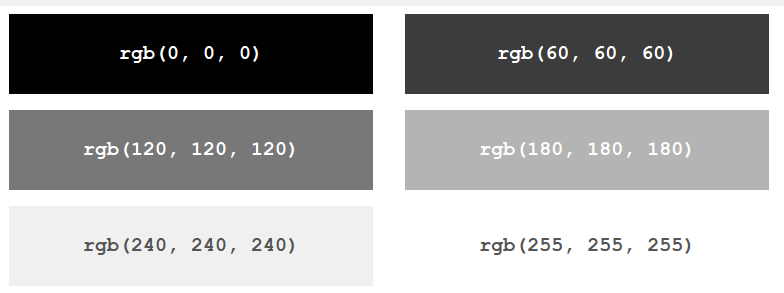
\includegraphics[height=0.4\paperheight]{fig/aula4/rgb.png} \\
		  \tiny Cores rgb.
	  \end{center}
	  \begin{center}
		\lstinputlisting[linerange={4-4}]{fig/aula3/color_elements.css}
		\tiny Exemplo de uso RGB
	\end{center}
	  
\end{frame}
%---------------------------------------------------------------------------------
\begin{frame}{Cores CSS - HEX}
É possível criar muitas cores utilizando Hexadecimal \#rrggbb\\
	\begin{center}
		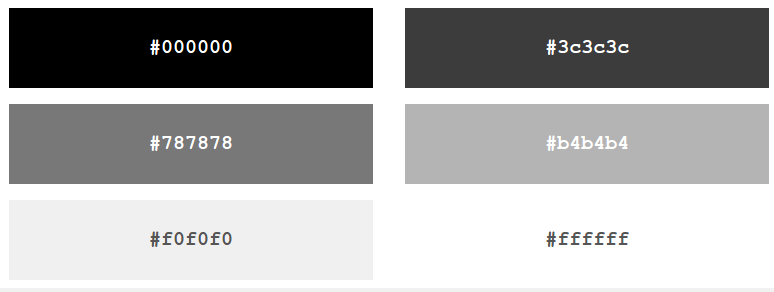
\includegraphics[height=0.4\paperheight]{fig/aula4/hex.png} \\
		\tiny Cores Hexadecimal.
	\end{center}
	\begin{center}
		\lstinputlisting[linerange={5-5}]{fig/aula3/color_elements.css}
		\tiny Exemplo de uso Hexadecimal
	\end{center}
	  
\end{frame}
%---------------------------------------------------------------------------------
\begin{frame}{Cores CSS - RGBA}
Precisa de transparência? rgba(\textcolor{red}{Red}, \textcolor{green}{Green}, \textcolor{blue}{Blue}, 
alpha)\\
	\begin{center}
		  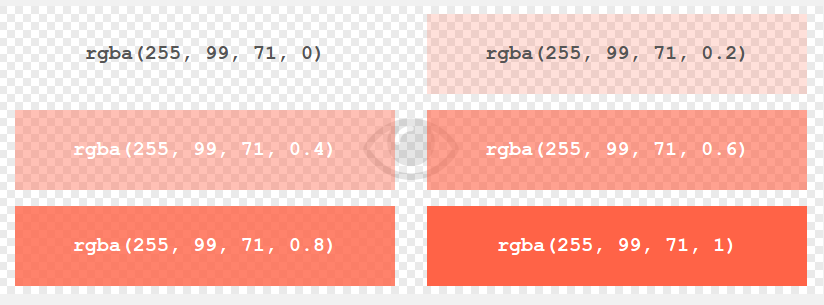
\includegraphics[height=0.4\paperheight]{fig/aula4/rgba.png} \\
		  \tiny Cores Hexadecimal.
	  \end{center}
	  \begin{center}
		\lstinputlisting[linerange={6-6}]{fig/aula3/color_elements.css}
		\tiny Exemplo de uso RGBA
	\end{center}
	  
\end{frame}
%---------------------------------------------------------------------------------
\begin{frame}{O poder das Cores CSS}
Colorindo elementos com CSS.\\
Crie uma página colors\_page.html com essa estrutura:
	\begin{center}
	 \lstinputlisting[linerange={21-28}]{fig/aula4/colors_page.html}
	\end{center}	  
\end{frame}
%---------------------------------------------------------------------------------
\begin{frame}{O poder das Cores CSS}
Acrescente este estilo:
	\begin{center}
	 \lstinputlisting[linerange={5-15}]{fig/aula4/colors_page.html}
	\end{center}	  
\end{frame}
%-------------------------------------------------------------------------------
\section{Formulário}
\begin{frame}{Formulários}
  \begin{itemize}
    \item Formulários são utilizados para a aquisição de informações do 
usuário;
      \item Um formulário é englobado pela tag: $<$form method = `` ''
action = `` ''$>$
     \item \textbf{method} define a forma de envio dos valores entre get 
ou post;
 \item \textbf{action} aponta para a página no servidor que receberá 
as informações do formulário;
\end{itemize}
\end{frame}
%-------------------------------------------------------------------------------
\begin{frame}{Input}
  Text e Password
    \begin{columns}
    \begin{column}{0.4 \textwidth}
      \small
     \begin{itemize}
       \item Adiciona uma caixa de inserção de texto (textfield);
        \item Parâmetros:
        \item \textbf{type};
        \item \textbf{name};
        \item \textbf{maxlength};
        \item \textbf{placeholder};
        \item \textbf{required};
     \end{itemize}
    \end{column}
    
    \begin{column}{0.5\textwidth}
     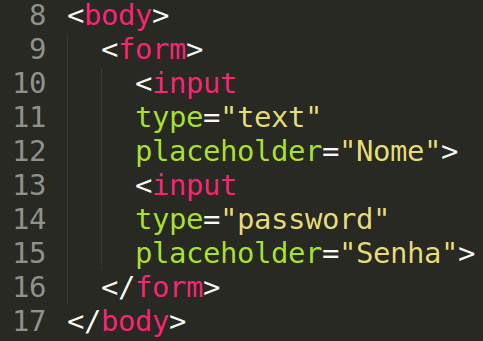
\includegraphics[height=0.45\paperheight]{fig/aula4/aula4_7.png}
    \end{column}
  \end{columns}
\end{frame}
%---------------------------------------------------------
\begin{frame}{TextArea}
    \begin{columns}
    \begin{column}{0.4 \textwidth}
      \small
      Adiciona uma caixa de inserção de textos longos;\\
      Parâmetros:
     \begin{itemize}
       \item col;
        \item row;
        \item name;
        \item placeholder;
        \item required;
     \end{itemize}
    \end{column}
    
    \begin{column}{0.5\textwidth}
     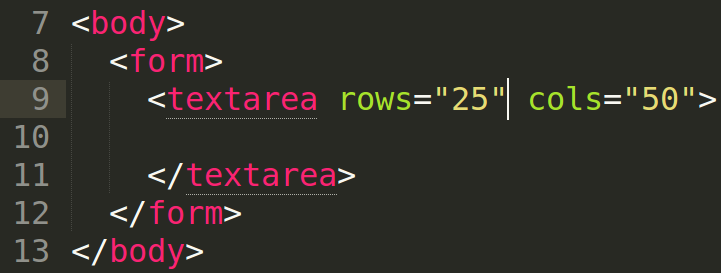
\includegraphics[height=0.25\paperheight]{fig/aula4/aula4_8.png}
    \end{column}
  \end{columns}
\end{frame}
%-------------------------------------------------------------------------------
\begin{frame}{Input Radio button}
  Adiciona um botão de opção única. Parâmetros:
    \begin{columns}
    \begin{column}{0.3 \textwidth}
      \small
     \begin{itemize}
       \item col;
        \item type;
        \item value;
        \item name;
        \item checked;
        \item required
     \end{itemize}
    \end{column}
    
    \begin{column}{0.6\textwidth}
     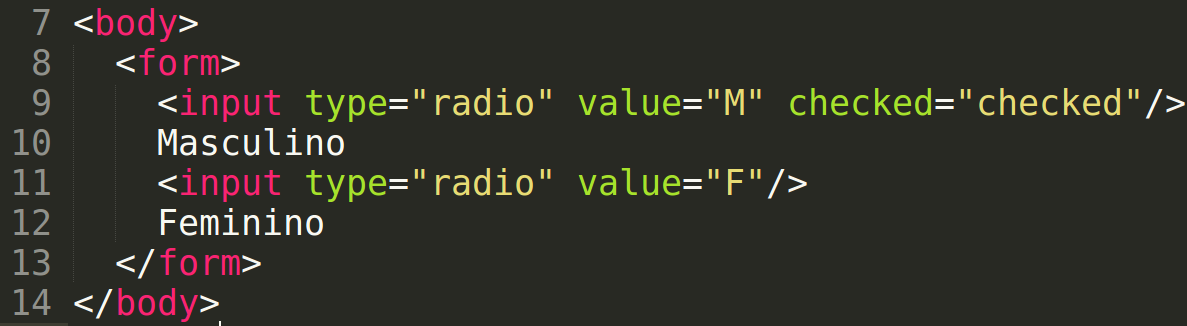
\includegraphics[height=0.2\paperheight]{fig/aula4/aula4_9.png}
    \end{column}
  \end{columns}
  
  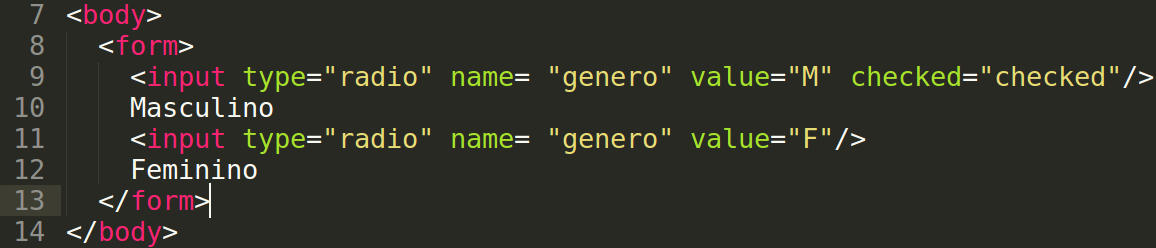
\includegraphics[height=0.2\paperheight]{fig/aula4/aula4_10.png}
\end{frame}
%-------------------------------------------------------------------------------
\begin{frame}{Input Check Box}
  Adiciona um botão de opção múltipla. \\Parâmetros:
    \begin{columns}
    \begin{column}{0.3 \textwidth}
      \small
     \begin{itemize}
       \item col;
        \item type;
        \item value;
        \item name;
        \item checked;
        \item required
     \end{itemize}
    \end{column}
    
    \begin{column}{0.6\textwidth}
     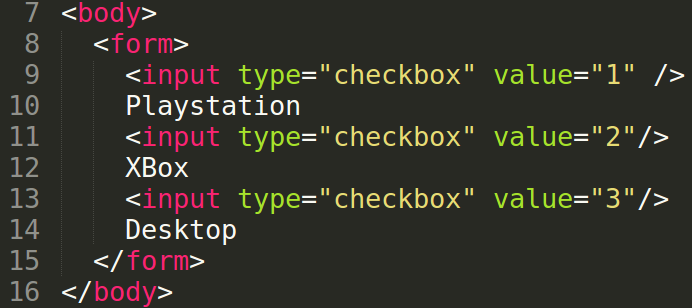
\includegraphics[height=0.35\paperheight]{fig/aula4/aula4_11.png}
    \end{column}
  \end{columns}
\end{frame}
%-------------------------------------------------------------------------------
\begin{frame}{DropDown}
  Adiciona uma lista suspensa. \\$<$select$>$: Parâmetros
    \begin{columns}
    \begin{column}{0.3 \textwidth}
      \small
     \begin{itemize}
       \item name;
        \item required;
     \end{itemize}
     $<$option$>$: Parâmetros
     \begin{itemize}
        \item value;
        \item selected;
        \item 
     \end{itemize}
    \end{column}
    
    \begin{column}{0.6\textwidth}
     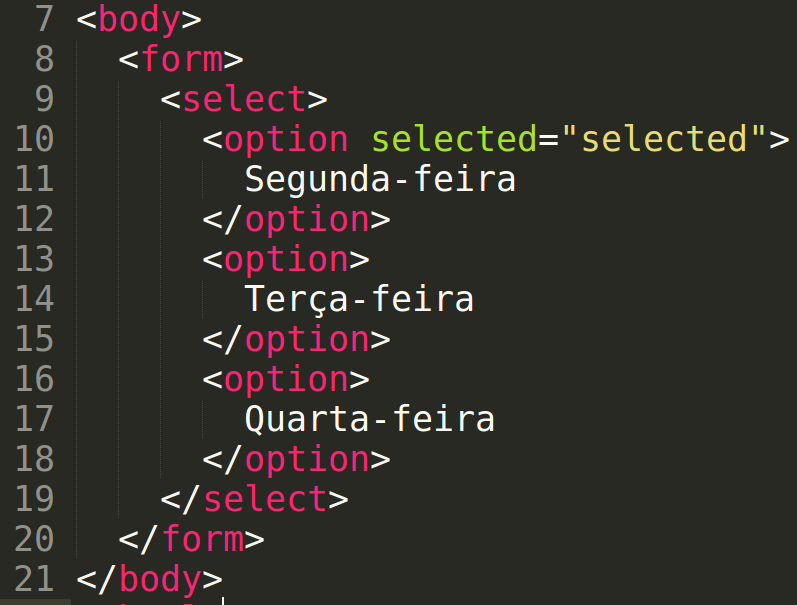
\includegraphics[height=0.5\paperheight]{fig/aula4/aula4_12.png}
    \end{column}
  \end{columns}
  \tiny{\textbf{Fonte:} \cite{wschool2021html}}.
\end{frame}
%-------------------------------------------------------------
\section{Atividades}
\begin{frame}{Atividade de aula}
\begin{enumerate}
 \item Crie uma página WEB de formulário, para cadastro de contatos.
 \item A página deve conter entradas de texto, raddio button, checkbox e DropDown.
  \item Acrescente estilo CSS a essa página;
\end{enumerate}
 
\end{frame}


%-----------------------------------------------------------------------------
%\section{Atividades}
%\begin{frame}{Atividade 1}
%Sobre barras de navegação. Vamos utilizar alguns conceitos conhecidos para criar uma barra de navegação 
%vertical.
%	\begin{center}
%		  \includegraphics[height=0.4\paperheight]{aep_1_2.png} \\
%	  \end{center}
%\end{frame}
%----------------------------------------------------------
%\begin{frame}{Atividade 2}
%Reproduza a página a seguir utilizando propriedades de borda;
%  \begin{center}
%    \includegraphics[height=0.2\paperheight]{AEP_1_1.png} \\
%  \end{center}
%\end{frame}

%-----------------------------------------------------------------------
\section{Leitura recomendada}
\begin{frame}{Leitura complementar}
 Para mais informações sobre HTML e CSS, leia:\\
 \begin{columns}
   \begin{column}{0.5\textwidth}
    Desenvolvimento de Software II: Introdução ao Desenvolvimento Web com HTML, CSS, JavaScript e PHP \\
     Capítulo 4 - Página 61\\ 
      \cite{miletto2014desenvolvimento}
   \end{column}
   \begin{column}{0.3\textwidth}
    \begin{center}
  
\includegraphics[height=0.45\paperheight]{fig/aula3/milleto2014.jpeg} \\
 \end{center}
   \end{column}
 \end{columns}
\end{frame}
%--------------------------aula 4 des. app---------------------------------------------

\section{Referências}
\begin{frame}{Referências}%[allowframebreaks]
\frametitle{Referências}
\small
\begin{center}
\tiny
\bibliographystyle{apalike}
\bibliography{ref_aula}
\end{center}
\end{frame}
 
\end{document}
